\documentclass[11pt]{article}

\usepackage{amsmath}
\usepackage{minted}
\usepackage{hyperref}
\usepackage[margin=2.0cm]{geometry}

\usepackage{graphicx}
\graphicspath{ {/home/ubuntu/www/octopress/source/} }

\def\title{Pricing Stock Options via the Binomial Model}
\newcommand{\Rev}{\text{rev}\;}
\newcommand\del[1]{\left(#1\right)}
\newcommand\nicefrac[2]{\frac{#1}{#2}}
\newcommand\set[1]{\left\{#1\right\}}
\newcommand\cF{\mathcal{F}}
\newcommand\Asterisk{*}


\setlength\parindent{1cm}

\begin{document}

Though most of us are familiar with stocks on the stock market, we may not be
quite as familiar with the derivatives that are traded on similar markets. One
such derivative is called an ``option''. Options are, essentially, the right to
buy or sell a stock at a given price. These two types of options are known as
``call'' and ``put'' options, respectively. For instance, I can buy a CALL
option for AAPL (Apple) with a strike price of \$430.30 dollars and an
expiration date of next Wednesday; this means that at any time before next
Wednesday, I can buy an AAPL stock at that price, regardless of what the price
of the stock (the spot price) currently is. If by next Wednesday the price has
risen to \$450, then I can buy for \$430.30 and sell for \$450, thus earning
myself a hefty profit. A PUT option is similar, but instead of being a bet on
rising value, it is a bet on falling value, and allows you to sell a stock for
a price higher than the spot price. Options are an incredibly fundamental derivatives,
with many traders using exclusively options for their activities. With this in
mind, a question arises very naturally: given some option, how much should I be
willing to pay in order to buy this option? Is the Apple CALL I described
previously worth \$1, or \$10? If Apple rising to \$450 is very likely, then
obviously the call must be more expensive, since it nets a profit of almost
\$20. However, if there is no chance whatsoever that Apple will rise above
\$430.30, the option is near-worthless.

One algorithm for pricing options is known as the Binomial Options Pricing
Model (BOPM for short). It assumes that the daily continuous growth rates for
the underlying stock are normally distributed around zero (the mean is $\alpha
= 0$) with some variance $\sigma^2$. Although these assumptions are not quite true,
they are close enough to true in certain circumstances to be useful.

Next, we assume that the stock price is a discrete-time process with some timestep
$\Delta t$, and that at each timestep the stock price goes up by a factor of $u$ or goes down by a
factor of $d = \nicefrac{1}{u}$. (Since going up by a factor of $u$ is an \emph{increase}, we
enforce that $u \ge 1$ and thus $d \in [0, 1]$.) These two factors come from the assumption that the
price is an Ito process with an $\alpha$ of zero.  Therefore, we can compute
the two factors from the volatility of the stock, and let
\begin{align*}
    u &= e^{\sigma\sqrt{\Delta t}} \\
    d &= e^{-\sigma\sqrt{\Delta t}}
\end{align*}
where $\sigma$ is the volatility and $\sqrt{\Delta t}$ is a time-adjustment
factor to scale the volatility by the timestep duration. 

Once we have computed $u$ and $d$, we can, starting at time $t = 0$, compute the possible stock
prices at times $t = k\Delta t$ for all $k$ starting from zero and going to the expiration date of
the option. We can build a tree with one node for each possible stock price at each timestep,
starting from $t = 0$ and $S = S_0$. The next timestep $t = \Delta t$ will then have two nodes, one
for $uS_0$ and one for $dS_0$. The timestep aftewards for $t = 2\Delta t$ will have (technically)
four nodes equal to $u^2S_0$, $udS_0$, $duS_0$, and $d^2S_0$. However, note that \(ud = du =
u\frac{1}{u} = 1,\) which means that we can collapse the internal nodes into one. Therefore, at time
$t=k\Delta t$, there will be a total of $k+1$ nodes, because you will have prices equal to $u^i
d^{k-i}S_0$ for every $i \in \set{0, 1, \cdots, k}$.

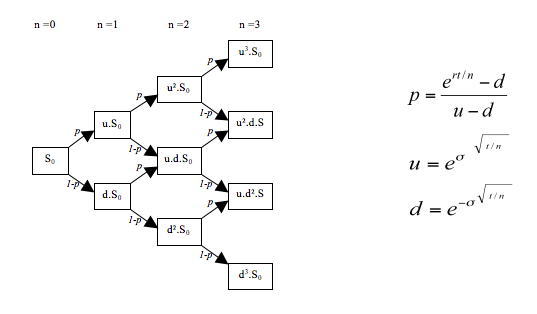
\includegraphics[scale=0.5]{images/bopm.png}\\
Binomial Options Pricing Model tree.

The ultimate goal of the binomial options pricing model is to compute the price of the option at
each node in this tree, eventually computing the value at the root of the tree. We begin by
computing the value at the leaves. The value at the leaves is easy to compute, since it is simply
the exercise value. If we let $K$ be the strike price of the option and let $S_n$ be the value of
the stock at the given node, then the price at the given node will be
\begin{align*}
    C &= \max \del{0, S_n - K} \qquad \text{(for a call option)} \\
    C &= \max \del{0, K - S_n} \qquad \text{(for a put option)} \\
\end{align*}
If the call or put options are unprofitable, they will simply be allowed to expire without
exercising, and thus will have a price of zero (will be a worthless option). (You can verify these
for a call option by noting that if the stock price is greater than the strike price, $S_n - K$ is
positive, so if it is a call option you would be able to buy the asset for $K$ and then sell it for
$S_n$, thus earning $S_n - K$ in profit.)

In order to proceed further, we need a method of computing the option price at the internal nodes of
the binomial model tree. For each internal node, we compute the ``binomial value'', which is the
time-decayed expected future payoff of the option. This is entirely logical, as if the option has an
expected price of $E[P]$ in a timestep of $\Delta t$, the current price is simply equal to the
backwards-discounted price of $e^{-r\Delta t} E[P]$, where $r$ is the risk free discount rate. The
expected value for future option price can be computed by examining the nodes closer to the leaves;
if we are at some stock price $S_i$, then the two possibilities for price evolution are $uS_i$ and
$dS_i$, and since those are farther down the tree, we have already computed the options prices for
these nodes. Therefore, the expected value of options price in one timestep is given by
\(E[P] = pC_\text{up} + (1-p)C_\text{down}\), where $C_\text{up}$ and $C_\text{down}$ are the
options prices for the nodes corresponding to the stock price going up or down in the timestep and
$p$ is the probability of the stock price going up. In choosing the probability $p$ to use, we wish
that $X \sim \text{Binom}(n, p)$ simulates the random geometric Brownian motion of a stock with
percentage volatility $\sigma$ and percentage drift $\mu$. Allowing for dividends with divident yield
$q$, this probability comes out to be $p = \frac{e^{(r-q)\Delta t} - d}{u - d}$. The value
\[e^{-r\Delta t}\del{pC_\text{up} + (1-p)C_\text{down}},\:\;p = \frac{e^{(r-q)\Delta t} - d}{u - d}\]
is known as the binomial value of the node and is a recurrence relation for computing the binomial
value of an internal node given the options price of its children farther down the tree. Since we
have a separate method of computing the prices of the leaves, we can then compute the binomial value
of any node in the tree. 

Note that though it may be tempting to say that the binomial value \emph{is}
the options price, this may not be the case; in American style options (the
type described at the start of this post), every node also has the option of
exercising the option, so the options price is the maximum of the binomial
value and the profit garnered by exercising the option at that point in time.
The profit may be assessed in exactly the same manner as the computation for
the leaves, with two cases, one for call and one for put options. However,
there exist European style options, where early exercise is not an option, so
the binomial value is the options price; similarly, there exist Bermudan style
options, where early exercise is only an option at some nodes, and only at
those nodes do you choose the maximum of the potential profit and the binomial
value. This demonstrates the flexibility of the binomial options pricing model,
and concludes the description of the separate pieces Binomial Options Pricing
Model algorithm. A very na\"{\i}ve yet correct Python implementation of this
algorithm is provided; although this algorithm is correct, it could be sped up
quite easily to run in $O(N^2)$ instead of $O(2^N)$ time via dynamic
programming techniques.

\newpage
\textbf{Binomial Options Pricing Model: Na\"{\i}ve Python Implementation} {\scriptsize \href{http://andrew.gibiansky.com/downloads/code/bopm.py}{(download)}}

\begin{minted}{python}
#!/usr/bin/env python
from math import exp

# Input stock parameters
dt = input("Enter the timestep: ")
S = input("Enter the initial asset price: ")
r = input("Enter the risk-free discount rate: ")
K = input("Enter the option strike price: ")
p = input("Enter the asset growth probability p: ")
u = input("Enter the asset growth factor u: ")
N = input("Enter the number of timesteps until expiration: ")

# Input whether this is a call or a put option
call = raw_input("Is this a call or put option? (C/P) ").upper().startswith("C")

def price(k, us):
    """ Compute the stock price after 'us' growths and 'k - us' decays. """
    return S * (u ** (2 * us - k))

def bopm(k, us):
    """
    Compute the option price for a node 'k' timesteps in the future
    and 'us' growth events. Note that thus there are 'k - us' decay events.
    """

    # Compute the exercise profit
    stockPrice = price(k, us)
    if call: exerciseProfit = max(0, stockPrice - K)
    else:    exerciseProfit = max(0, K - stockPrice)

    # Base case (this is a leaf)
    if k == N: return exerciseProfit

    # Recursive case: compute the binomial value 
    decay = exp(-r * dt)
    expected = p * bopm(k + 1, us + 1) + (1 - p) * bopm(k + 1, us)
    binomial = decay * expected

    # Assume this is an American-style option
    return max(binomial, exerciseProfit)

print 'Computed option price: $%.2f' % bopm(0, 0)
\end{minted}

\end{document}
